\numoptstrue
\yearpaper{2026}{Day 1 \textperiodcentered{} First Session \textperiodcentered{} Version A1 \textperiodcentered{} 60 Questions \textperiodcentered{} 60 Marks \textperiodcentered{} 80 Minutes}{}
\begin{multicols}{2}

\QQ{Match the physical quantities given in List-I with dimensions expressed in terms of mass (M), length (L), time (T) and electric current (A) given in List-II.\par
\smallskip
\begin{tabular}{@{}ll@{\hspace{1.2em}}ll@{}}
\multicolumn{2}{@{}l}{\textit{List-I}} & \multicolumn{2}{l}{\textit{List-II}}\\
(a) & Torque & (i) & $[\mathrm{M^{-1}L^{-2}T^{4}A^{2}}]$\\
(b) & Gravitational constant & (ii) & $[\mathrm{M^{1}L^{2}T^{-1}}]$\\
(c) & Capacitance & (iii) & $[\mathrm{M^{-1}L^{3}T^{-2}}]$\\
(d) & Planck's constant & (iv) & $[\mathrm{M^{1}L^{2}T^{-2}}]$
\end{tabular}\par\smallskip Codes:\ntag{A}{8}{keph101}{8}{}{Class XI Part 1 \textperiodcentered{} Ch 1}\nsrc{JEE Main 2021 (25 Feb, Shift 1) -- match-the-list of dimensions ($h$, $E$, $V$, $p$)}}
{\opt{a--iv, b--ii, c--iii, d--i}{a--iv, b--iii, c--i, d--ii}{a--iv, b--i, c--iii, d--ii}{a--ii, b--i, c--iii, d--iv}}

\QQ{A car covers the first half of the distance between two places at $40\unit{km/h}$ and another half at $50\unit{km/h}$. The average speed of the car is\ntag{A}{15}{keph102}{3}{}{Class XI Part 1 \textperiodcentered{} Ch 2}\nsrc{NEET 2023 -- average speed, half distance at 8 and half at 20}}
{\opt{$45.00\unit{km/h}$}{$44.44\unit{km/h}$}{$43.14\unit{km/h}$}{$42.04\unit{km/h}$}}

\QQ{Two bodies are projected with the same velocity. If one is projected at an angle of $30^\circ$ and the other at $45^\circ$ to the horizontal, then the ratio of maximum heights attained is
\fig{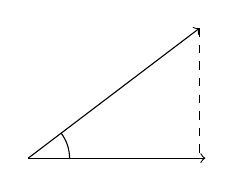
\begin{tikzpicture}[scale=0.75]
\draw[->] (0,0) -- (3,0);
\draw[->] (0,0) -- (2.9,2.2);
\draw[dashed] (2.9,2.2) -- (2.9,0);
\draw (0.7,0) arc (0:37:0.7);
\end{tikzpicture}}\ntag{D}{39}{keph103}{13}{}{Class XI Part 1 \textperiodcentered{} Ch 3}}
{\opt{3:1}{1:2}{4:1}{1:3}}

\QQ{The velocity of a particle moving along $x$-axis is given as $V = x^2 - 5x + 4$ (in m/s) where $x$ denotes the $x$-coordinate of the particle in metres. The magnitude of the acceleration of the particle when the velocity of the particle is zero is\ntag{A}{18}{keph102}{6}{}{Class XI Part 1 \textperiodcentered{} Ch 2}\nsrc{JEE Main 2024 (1 Feb, Shift 2), $v=4\sqrt{x}$; AIEEE 2006, $v=\alpha\sqrt{x}$ -- acceleration from $v(x)$}}
{\opt{$2\unit{m/s^2}$}{$3\unit{m/s^2}$}{Zero}{$1\unit{m/s^2}$}}

\QQ{A man weighs $80\unit{kg}$. He stands on a weighing scale in a lift which is moving upwards with a uniform acceleration of $6\unit{m/s^2}$. What would be his weight in kg? ($g = 10\unit{m/s^2}$)\ntag{D}{69}{keph104}{21}{ \textperiodcentered{} Exercise 4.13}{Class XI Part 1 \textperiodcentered{} Ch 4}}
{\opt{Zero}{$48\unit{kg}$}{$120\unit{kg}$}{$128\unit{kg}$}}

\QQ{A mass M is hung with a light inextensible string as shown in figure. Find the tension of the horizontal string.
\fig{\begin{tikzpicture}[scale=0.8]
\fill[pattern=north east lines] (0.9,2.5) rectangle (2.6,2.65);
\draw (0.9,2.5) -- (2.6,2.5);
\fill[pattern=north east lines] (-1.65,-0.8) rectangle (-1.5,1.2);
\draw (-1.5,-0.8) -- (-1.5,1.2);
\draw (0,0) -- (1.8,2.5) node[pos=0.55,sloped]{\tikz\draw[-{Stealth[length=4pt]}] (0,0)--(0.01,0);};
\draw (0,0) -- (-1.5,0) node[pos=0.5]{\tikz\draw[-{Stealth[length=4pt]}] (0.01,0)--(0,0);};
\draw (0,0) -- (0,-1.2) node[pos=0.5]{\tikz\draw[-{Stealth[length=4pt]}] (0,0.01)--(0,0);};
\draw (1.8,2.5) ++(-0.4,0) arc (180:234:0.4);
\node[lbl] at (1.15,2.2) {$45^\circ$};
\node[lbl,right] at (0,0) {O};
\draw[pattern=north east lines] (-0.25,-1.2) rectangle (0.25,-1.55);
\node[lbl,right] at (0.3,-1.38) {M};
\end{tikzpicture}}\ntag{D}{58}{keph104}{10}{ \textperiodcentered{} Example 4.6}{Class XI Part 1 \textperiodcentered{} Ch 4}}
{\opt{$\sqrt2\,Mg$}{$\sqrt3\,Mg$}{$Mg$}{$3\,Mg$}}

\QQ{Two bodies with kinetic energies in the ratio of 3:1 are moving with equal linear momentum. The ratio of their masses is\ntag{A}{73}{keph105}{3}{}{Class XI Part 1 \textperiodcentered{} Ch 5}\nsrc{JEE Main 2021 (24 Feb, Shift 2) -- equal momentum, ratio of kinetic energies}}
{\opt{1:4}{1:3}{1:2}{1:1}}

\QQ{A horizontal force of $5\unit{N}$ is applied on a stationary body of mass $5\unit{kg}$, which is initially at rest on a frictionless table. The change in kinetic energy of the body in $10\unit{s}$ is\ntag{A}{73}{keph105}{3}{}{Class XI Part 1 \textperiodcentered{} Ch 5}\nsrc{None found in NEET/AIPMT/AIEEE/JEE papers, 2005--2026 (NCERT concept application)}}
{\opt{$25\unit{J}$}{Zero}{$125\unit{J}$}{$250\unit{J}$}}

\QQ{The angular momentum of a moving body remains constant, if\ntag{D}{108}{keph106}{17}{}{Class XI Part 1 \textperiodcentered{} Ch 6}}
{\opt{net external force is applied}{net pressure is applied}{net external torque is applied}{net external torque is not applied}}

\QQ{If the earth were to suddenly contract to half of its present radius, what would be the duration of the day?\ntag{A}{122}{keph106}{31}{}{Class XI Part 1 \textperiodcentered{} Ch 6}\nsrc{JEE Main 2024 (6 Apr, Shift 1) -- earth's radius reduced, new length of day}}
{\opt{$6\unit{h}$}{$18\unit{h}$}{$24\unit{h}$}{$30\unit{h}$}}

\QQ{Imagine a new planet having the same density as that of the earth, but it is two times bigger than the earth in size. If the acceleration due to gravity on the surface of the earth is $g$ and that on the surface of the new planet is $g'$, then\ntag{A}{132}{keph107}{6}{}{Class XI Part 1 \textperiodcentered{} Ch 7}\nsrc{NEET 2016 (Phase I) -- planet with radius and density twice that of earth}}
{\opt{$g' = \dfrac{g}{4}$}{$g' = 8g$}{$g' = 2g$}{$g' = 4g$}}

\QQ{Suppose the acceleration due to gravity at the earth's surface is $g\unit{m/s^2}$ and at the surface of moon it is $g'\unit{m/s^2}$. An M kg passenger goes from the earth to the moon in a spaceship moving with a constant velocity (Neglect all other objects in the sky). Which curve best represents the weight (net gravitational force) as a function of time?
\fig{\begin{tikzpicture}[scale=0.9]
\draw[->] (0,0) -- (3.3,0) node[right,lbl]{$t$};
\draw[->] (0,0) -- (0,2.4);
\node[lbl,below left] at (0,0) {O};
\node[lbl,left] at (0,2) {$Mg$};
\node[lbl,left] at (0,1.2) {$Mg'$};
\draw[dashed] (0,1.2) -- (2.6,1.2) -- (2.6,0) node[below,lbl]{$t_0$};
\draw (0,2) -- (2.6,1.2) node[pos=0.35,above,lbl]{A};
\draw (0,2) .. controls (0.6,1.3) and (1.4,1.2) .. (2.6,1.2);
\node[lbl] at (1.0,1.5) {B};
\draw plot[smooth,tension=0.7] coordinates {(0,2)(0.45,0.85)(1.2,0.32)(1.95,0.55)(2.6,1.2)};
\node[lbl] at (1.55,0.62) {C};
\draw plot[smooth,tension=0.7] coordinates {(0,2)(0.35,0.7)(1.2,0.0)(2.0,0.4)(2.6,1.2)};
\node[lbl] at (0.95,-0.18) {D};
\end{tikzpicture}}\ntag{A}{132}{keph107}{6}{}{Class XI Part 1 \textperiodcentered{} Ch 7}\nsrc{None found in NEET/AIPMT/AIEEE/JEE papers, 2005--2026 (NCERT concept application)}}
{\opt{A}{B}{C}{D}}

\QQ{Instrument fitted in the carburetor of the automobile to provide the correct mixture of air and fuel necessary for combustion works on\ntag{A}{187}{keph202}{8}{}{Class XI Part 2 \textperiodcentered{} Ch 9}\nsrc{NEET 2023 -- ``The venturi-meter works on: Bernoulli's principle''}}
{\opt{Pascal's Law}{Bernoulli's Principle}{Newton's Law of Cooling}{Archimedes' Principle}}

\QQ{There are two wires of same material and same length while the diameter of second wire is two times the diameter of the first wire. Then the ratio of extensions produced in the wires by applying same load will be\ntag{D}{170}{keph201}{4}{}{Class XI Part 2 \textperiodcentered{} Ch 8}}
{\opt{1:1}{1:2}{2:1}{4:1}}

\QQ{In a capillary tube experiment, a vertical $30\unit{cm}$ long capillary tube is dipped in water, water rises upto a height of $10\unit{cm}$ due to capillarity. If this experiment is conducted in a freely falling elevator, then the length of the water column becomes\ntag{A}{197}{keph202}{18}{}{Class XI Part 2 \textperiodcentered{} Ch 9}\nsrc{AIEEE 2005 -- capillary tube in a freely falling elevator (20 cm tube, 8 cm rise)}}
{\opt{$10\unit{cm}$}{$20\unit{cm}$}{$30\unit{cm}$}{Zero}}

\QQ{In thermodynamic processes, which of the following statements is not true?\ntag{D}{234}{keph204}{9}{}{Class XI Part 2 \textperiodcentered{} Ch 11}}
{\opt{In an isothermal process, the temperature remains constant}{In an isobaric process, the volume remains constant}{In an adiabatic process, the system is insulated from the surroundings}{In an adiabatic process, $PV^{\gamma} =$ a constant}}

\QQ{The graph of pressure $P$ and volume $V$ of 1 mole of an ideal gas at constant temperature is\ntag{D}{234}{keph204}{9}{}{Class XI Part 2 \textperiodcentered{} Ch 11}}
{\optfig{\gaxes{$V$}{$P$}{\draw (0,1.1) -- (1.7,1.1);}}
        {\gaxes{$V$}{$P$}{\draw (0,0) -- (1.5,1.5);}}
        {\gaxes{$V$}{$P$}{\draw (0.3,1.5) -- (1.6,0.25);}}
        {\gaxes{$V$}{$P$}{\draw[domain=0.25:1.9,samples=40] plot (\x,{0.38/\x});}}}

\QQ{A mass of $1\unit{kg}$ is executing SHM. Its displacement is given by $x = 6.0\cos(100t + \pi/4)\unit{cm}$. What is the maximum kinetic energy?\ntag{D}{268}{keph206}{10}{}{Class XI Part 2 \textperiodcentered{} Ch 13}}
{\opt{$3\unit{J}$}{$6\unit{J}$}{$9\unit{J}$}{$18\unit{J}$}}

\QQ{A source of frequency $\nu$ gives 6 beats/second when sounded with a source of frequency $200\unit{Hz}$. The second harmonic of frequency $2\nu$ of the source gives 8 beats/second when sounded with a source of frequency $420\unit{Hz}$. The value of $\nu$ is\ntag{A}{294}{keph207}{17}{}{Class XI Part 2 \textperiodcentered{} Ch 14}\nsrc{NEET 2013 -- beats with 250 Hz; second harmonic gives beats with 513 Hz}}
{\opt{$205\unit{Hz}$}{$206\unit{Hz}$}{$195\unit{Hz}$}{$210\unit{Hz}$}}

\QQ{Following are statements of a few processes taking place in nature.\par
\begin{stmts}
\item Free expansion of a gas
\item The combustion of a mixture of petrol and air ignited by a spark
\item The leaking of gas from the kitchen cylinder
\item The transfer of heat from one heated part of a liquid to the other colder part
\end{stmts}\par
Which amongst these processes are irreversible in nature?\ntag{D}{236}{keph204}{11}{}{Class XI Part 2 \textperiodcentered{} Ch 11}}
{\opt{I and II}{III and IV}{II, III and IV}{I, II, III and IV}}

\QQ{An electron falls through a distance of $1.5\unit{cm}$ in a uniform electric field of magnitude $2.0\times10^{4}\unit{N/C}$ from rest. The time taken to cover this distance in second is \rule{1.2cm}{0.4pt} ($e = 1.6\times10^{-19}\unit{C}$, $m_e = 9.11\times10^{-31}\unit{kg}$)\ntag{D}{17}{leph101}{17}{ \textperiodcentered{} Example 1.7}{Class XII Part 1 \textperiodcentered{} Ch 1}}
{\opt{$2.9\times10^{-9}$}{$2.9\times10^{9}$}{$4\times10^{-6}$}{$4\times10^{6}$}}

\QQ{What will be the total electric flux through the faces of the cube as given in the figure with side of length `$a$' if a charge $Q$ is placed at B, midpoint of an edge of the cube (see figure)?
\fig{\begin{tikzpicture}[scale=0.85]
\draw (0,0) rectangle (1.6,1.6);
\draw (0,1.6) -- (0.75,2.35) -- (2.35,2.35) -- (1.6,1.6);
\draw (2.35,2.35) -- (2.35,0.75) -- (1.6,0);
\fill (1.975,0.375) circle (1.6pt);
\node[lbl,above left] at (1.975,0.375) {$Q$};
\node[lbl,right] at (1.975,0.3) {B};
\node[lbl,below] at (0.8,0) {$a$};
\end{tikzpicture}}\ntag{A}{29}{leph101}{29}{ \textperiodcentered{} Exemplar 1.19}{Class XII Part 1 \textperiodcentered{} Ch 1}\nsrc{None found in NEET/AIPMT/AIEEE/JEE papers, 2005--2026 (NCERT concept application)}}
{\opt{$\dfrac{Q}{8\varepsilon_0}$}{$\dfrac{Q}{3\varepsilon_0}$}{$\dfrac{Q}{4\varepsilon_0}$}{$\dfrac{Q}{2\varepsilon_0}$}}

\QQ{Consider three point charges $-2Q$, $Q$ and $-Q$ and three surfaces $S_1$, $S_2$ and $S_3$ as shown in the figure. Match the entries of List-I with that of List-II.\par\smallskip
\begin{matchtab}
\multicolumn{2}{@{}l}{\textit{List-I}} & \multicolumn{2}{l}{\textit{List-II}}\\[2pt]
(a) & Net flux through $S_1$ & (i) & $-2Q/\varepsilon_0$\\[2pt]
(b) & Net flux through $S_2$ & (ii) & $-Q/\varepsilon_0$\\[2pt]
(c) & Net flux through $S_3$ & (iii) & Zero
\end{matchtab}
\fig{\begin{tikzpicture}[scale=0.62]
\draw (0,0) ellipse (1.55 and 2.0);
\draw (0,0.75) circle (1.0);
\draw (0,-0.75) circle (1.0);
\fill (-0.25,1.25) circle (2pt) node[right,lbl]{$-2Q$};
\fill (-0.25,0) circle (2pt) node[right,lbl]{$Q$};
\fill (-0.25,-1.2) circle (2pt) node[right,lbl]{$-Q$};
\node[lbl] at (0.85,1.55) {$S_1$};
\node[lbl] at (0.95,-0.15) {$S_2$};
\node[lbl] at (1.3,-1.45) {$S_3$};
\end{tikzpicture}}\par Codes:\ntag{D}{29}{leph101}{29}{}{Class XII Part 1 \textperiodcentered{} Ch 1}}
{\opt{a--ii, b--i, c--iii}{a--iii, b--ii, c--i}{a--i, b--ii, c--iii}{a--ii, b--iii, c--i}}

\QQ{A parallel plate capacitor has a uniform electric field `$E$' in the space between the plates. If the distance between the plates is `$d$' and area of each plate is `$A$', the energy stored in the capacitor is\ntag{D}{74}{leph102}{30}{}{Class XII Part 1 \textperiodcentered{} Ch 2}}
{\opt{$\dfrac12\epsilon_0E^2$}{$\epsilon_0EAd$}{$\dfrac12\epsilon_0E^2Ad$}{$\dfrac{E^2Ad}{\epsilon_0}$}}

\QQ{In the circuit shown in the figure, the potential difference across the $4\,\mu\mathrm{F}$ capacitor is
\fig{\begin{circuitikz}[scale=0.62,transform shape]

\draw (0,2) to[C,l=$4\,\mu\mathrm{F}$] (2.6,2);
\draw (2.6,2) -- (2.6,3) to[C,l=$9\,\mu\mathrm{F}$] (5,3) -- (5,2);
\draw (2.6,2) -- (2.6,1) to[C,l=$3\,\mu\mathrm{F}$] (5,1) -- (5,2);
\draw (5,2) -- (6,2) -- (6,0) to[battery1,l=$12\,\mathrm{V}$] (0,0) -- (0,2);
\end{circuitikz}}\ntag{A}{71}{leph102}{27}{}{Class XII Part 1 \textperiodcentered{} Ch 2}\nsrc{None found in NEET/AIPMT/AIEEE/JEE papers, 2005--2026 (NCERT concept application)}}
{\opt{$3\unit{V}$}{$4\unit{V}$}{$9\unit{V}$}{$12\unit{V}$}}

\QQ{An electric dipole of dipole moment $\vec P$ is placed in the uniform electric field $\vec E$. Then which of the following statements are correct?\par
Statement I: The torque on the dipole is $\vec P\times\vec E$\par
Statement II: The potential energy of the dipole is $-\vec P\cdot\vec E$\par
Statement III: The net force on the dipole is non zero\ntag{D}{60}{leph102}{16}{}{Class XII Part 1 \textperiodcentered{} Ch 2}}
{\opt{I, II and III}{I and II only}{II and III only}{I and III only}}

\QQ{A $200\unit{J}$ of work is done in moving a charge $5\unit{C}$ from a point A where the potential is $-20\unit{V}$ to another point B where potential is $V$ volt. The value of $V$ at B is\ntag{D}{46}{leph102}{2}{}{Class XII Part 1 \textperiodcentered{} Ch 2}}
{\opt{$10\unit{V}$}{$20\unit{V}$}{$40\unit{V}$}{$60\unit{V}$}}

\QQ{In the figure, the values of currents $I_1$, $I_2$ and $I_3$ respectively are
\fig{\begin{circuitikz}[scale=0.72,transform shape,font=\large]
\draw (0,3) to[R,i>^=$5\,\mathrm{A}$] (2.2,3) to[R,i>^=$I_1$] (4.4,3) to[R,i>^=$1.5\,\mathrm{A}$] (6.6,3);
\draw (2.2,3) -- (2.2,1.3) to[R,i>_=$1\,\mathrm{A}$] (0,1.3);
\draw (4.4,3) to[R,i>^=$I_2$] (4.4,1.3) to[R,i>^=$1.5\,\mathrm{A}$] (6.6,1.3);
\draw (4.4,1.3) to[R,i>^=$I_3$] (4.4,-0.4);
\fill (2.2,3) circle (2pt) (4.4,3) circle (2pt) (4.4,1.3) circle (2pt);
\end{circuitikz}}\ntag{A}{97}{leph103}{17}{}{Class XII Part 1 \textperiodcentered{} Ch 3}\nsrc{None found in NEET/AIPMT/AIEEE/JEE papers, 2005--2026 (NCERT concept application)}}
{\opt{6\,A, 1.5\,A and 1\,A}{4\,A, 2.5\,A and 2\,A}{4\,A, 2.5\,A and 1\,A}{6\,A, 4.5\,A and 1.5\,A}}

\QQ{The number of electrons moving per second through the filament of a lamp of $60\unit{W}$ operating at $120\unit{V}$ is nearly ($e = 1.6\times10^{-19}\unit{C}$) \rule{1cm}{0.4pt}\ntag{A}{82}{leph103}{2}{}{Class XII Part 1 \textperiodcentered{} Ch 3}\nsrc{JEE Main 2024 (6 Apr, Shift 2) -- electrons per second in a 110 W, 220 V filament}}
{\opt{$6.2\times10^{18}$}{$6.2\times10^{19}$}{$3.1\times10^{18}$}{$3.1\times10^{19}$}}

\QQ{Given below are two statements:\par
Statement I: The resistivity of a conductor is independent of its temperature\par
Statement II: The resistivity of a semiconductor decreases with increase in temperature\par
Select the correct option.\ntag{D}{90}{leph103}{10}{}{Class XII Part 1 \textperiodcentered{} Ch 3}}
{\opt{Both Statement I and Statement II are false}{Both Statement I and Statement II are true}{Statement I is true but Statement II is false}{Statement I is false but Statement II is true}}

\QQ{Current flowing through a wire decreases linearly from $10\unit{A}$ to zero in $4\unit{s}$ as shown in the graph. Find the total charge flowing through the wire in the given time interval.
\fig{\begin{tikzpicture}[scale=0.55]
\draw[->] (0,0) -- (4.2,0) node[right,lbl]{$t$ (s)};
\draw[->] (0,0) -- (0,3.6) node[above,lbl]{$I$ (A)};
\draw (0,3) -- (2.8,0);
\draw (-0.1,3) -- (0.1,3) node[left=3pt,lbl]{10};
\node[lbl,below] at (2.8,0) {4};
\node[lbl,below left] at (0,0) {0};
\end{tikzpicture}}\ntag{A}{82}{leph103}{2}{}{Class XII Part 1 \textperiodcentered{} Ch 3}\nsrc{None found in NEET/AIPMT/AIEEE/JEE papers, 2005--2026 (NCERT concept application)}}
{\opt{$40\unit{C}$}{$20\unit{C}$}{$10\unit{C}$}{$80\unit{C}$}}

\QQ{In a conducting region, $10^{19}$ electrons and $10^{19}$ protons move to the left, while $10^{19}$ $\alpha$-particles move to the right per second. The resulting electric current is ($e = 1.6\times10^{-19}\unit{C}$) \rule{1cm}{0.4pt}\ntag{D}{81}{leph103}{1}{}{Class XII Part 1 \textperiodcentered{} Ch 3}}
{\opt{$3.2\unit{A}$ towards left}{$3.2\unit{A}$ towards right}{$1.6\unit{A}$ towards left}{$1.6\unit{A}$ towards right}}

\QQ{A point charge is placed in a moving train. A passenger A sitting in the train and person B on the ground observe the fields due to this charge. Then\ntag{A}{108}{leph104}{2}{}{Class XII Part 1 \textperiodcentered{} Ch 4}\nsrc{None found in NEET/AIPMT/AIEEE/JEE papers, 2005--2026 (NCERT concept application)}}
{\opt{A observes both electric and magnetic fields}{B observes both electric and magnetic fields}{A observes only magnetic field}{B observes only electric field}}

\QQ{A proton, an electron and an $\alpha$-particle enter at right angles to a uniform magnetic field with the same velocity. If $R_p$, $R_e$ and $R_\alpha$ are the radii of circular paths of these particles, then\ntag{D}{112}{leph104}{6}{}{Class XII Part 1 \textperiodcentered{} Ch 4}}
{\opt{$R_\alpha = R_p = R_e$}{$R_\alpha > R_p > R_e$}{$R_\alpha < R_p < R_e$}{$R_\alpha > R_p = R_e$}}

\QQ{Biot--Savart law indicates that an electron moving with a velocity $\vec V$ produces a magnetic field $\vec B$ around it such that\ntag{D}{113}{leph104}{7}{}{Class XII Part 1 \textperiodcentered{} Ch 4}}
{\opt{$\vec B$ is parallel to $\vec V$}{$\vec B$ is perpendicular to $\vec V$}{$\vec B$ is anti-parallel to $\vec V$}{$\vec B$ is inclined to $\vec V$ by $45^\circ$}}

\QQ{Two identical circular current loops carrying equal currents are placed with their axes inclined at $45^\circ$ to each other as shown in the figure. The resultant magnetic field at P is
\fig{\begin{tikzpicture}[scale=0.9]
\coordinate (P) at (2.2,0);
\coordinate (C1) at (0,0);
\coordinate (C2) at ($(P)+(-135:2.2)$);
\draw[dashed] (C1) -- (P) node[pos=0.55,above,lbl]{$\sqrt3R$};
\draw[dashed] (C2) -- (P) node[pos=0.5,below right,lbl]{$\sqrt3R$};
\draw (C1) ellipse (0.35 and 0.85);
\draw[->] (-0.33,-0.3) -- (-0.3,-0.45);
\node[lbl] at (-0.6,-0.6) {$I$};
\draw (C1) -- (0,0.85) node[pos=0.5,right,lbl,inner sep=1pt]{$R$};
\draw[rotate around={45:(C2)}] (C2) ellipse (0.35 and 0.85);
\node[lbl] at ($(C2)+(-0.85,-0.55)$) {$I$};
\draw ($(P)+(-0.55,0)$) arc (180:225:0.55);
\node[lbl] at ($(P)+(-0.95,-0.32)$) {$45^\circ$};
\node[lbl,right] at (P) {P};
\draw[->] (3.6,0.2) -- (3.6,1.3) node[above,lbl]{Y};
\draw[->] (3.6,0.2) -- (4.7,0.2) node[right,lbl]{X};
\end{tikzpicture}}\ntag{A}{115}{leph104}{9}{}{Class XII Part 1 \textperiodcentered{} Ch 4}\nsrc{None found in NEET/AIPMT/AIEEE/JEE papers, 2005--2026 (NCERT concept application)}}
{\opt{$\dfrac{\mu_0I}{16\sqrt2R}\big[(\sqrt2+1)\hat i+\hat j\big]$}{$\dfrac{\mu_0I}{16\sqrt2R}\big[\sqrt2\,\hat i+\hat j\big]$}{$\dfrac{\mu_0I}{16R}\big[(\sqrt2+1)\hat i+\hat j\big]$}{$\dfrac{\mu_0I}{16R}\big[\sqrt2\,\hat i+\hat j\big]$}}

\QQ{If a paramagnetic bar is brought near a bar magnet, then it is\ntag{D}{148}{leph105}{13}{}{Class XII Part 1 \textperiodcentered{} Ch 5}}
{\opt{Attracted by both the poles of the bar magnet}{Repelled by both the poles of the bar magnet}{Attracted by the South-pole and repelled by the North-pole of the bar magnet}{Attracted by the North-pole and repelled by the South-pole of the bar magnet}}

\QQ{Pick out the WRONG statements about magnetic substances ($\chi$ = magnetic susceptibility) ($\mu_r$ = relative permeability).
\begin{stmts}
\item Substances with $-1\le\chi<0$ are diamagnetic
\item Substances with $\chi\gg1$ are paramagnetic
\item Substances with $\chi\ll1$ are ferromagnetic
\item Substances with $\mu_r\gg1$ are ferromagnetic
\end{stmts}\ntag{D}{147}{leph105}{12}{}{Class XII Part 1 \textperiodcentered{} Ch 5}}
{\opt{I and II}{III and IV}{II and III}{II and IV}}

\QQ{Work function of the metal is\ntag{D}{275}{leph203}{2}{}{Class XII Part 2 \textperiodcentered{} Ch 11}}
{\opt{Maximum possible energy acquired by an electron}{Equal for all metals}{Minimum energy required by an electron to just eject from metal surface}{Maximum energy which is given to electron to move out of metal surface}}

\QQ{Variation of photoelectric current with anode potential is shown below. Choose the correct option ($V_0$ = stopping potential). (Vertical axis: photoelectric current; horizontal axis: anode potential.)\ntag{D}{278}{leph203}{5}{}{Class XII Part 2 \textperiodcentered{} Ch 11}}
{\optfig{\begin{tikzpicture}[scale=0.5]\draw[->] (-1.3,0)--(2.4,0);\draw[->](0,-0.3)--(0,2.2);\draw (-1,0.08)--(-1,-0.08) node[below,lbl]{$V_0$};
 \draw (-1,0) .. controls (-0.3,0.2) and (0,1.4) .. (0.8,1.5) -- (1.9,1.45);\end{tikzpicture}}
{\begin{tikzpicture}[scale=0.5]\draw[->] (-1.3,0)--(2.4,0);\draw[->](0,-0.3)--(0,2.2);\draw (-1,0.08)--(-1,-0.08) node[below,lbl]{$V_0$};
 \draw (-1,0) -- (1.2,2.1);\end{tikzpicture}}
{\begin{tikzpicture}[scale=0.5]\draw[->] (-1.3,0)--(2.4,0);\draw[->](0,-0.3)--(0,2.2);\draw (-1,0.08)--(-1,-0.08) node[below,lbl]{$V_0$};
 \draw (0,1.3) -- (1.1,0);\end{tikzpicture}}
{\begin{tikzpicture}[scale=0.5]\draw[->] (-1.3,0)--(2.4,0);\draw[->](0,-0.3)--(0,2.2);\draw (-1,0.08)--(-1,-0.08) node[below,lbl]{$V_0$};
 \draw (0,0) .. controls (0.9,0.3) and (1.4,0.7) .. (1.65,2.1);\end{tikzpicture}}}

\QQ{In Faraday--Henry's experiment, a coil is connected to a galvanometer. For the deflection of pointer in the galvanometer, which of the following statement/s is/are WRONG?\par
The pointer in the galvanometer deflects --
\begin{stmts}[(\alph*)]
\item When the bar magnet is moved towards the stationary coil along its axis
\item When the bar magnet is moved away from the stationary coil along its axis
\item When the coil is moved towards the stationary bar magnet along its axis
\item When the coil and the magnet are moved without relative motion between them
\end{stmts}\ntag{D}{155}{leph106}{2}{}{Class XII Part 1 \textperiodcentered{} Ch 6}}
{\opt{a and b}{b and c}{a, b and c}{Only d}}

\QQ{In the figure shown, the conductor PQ of length $l$ is moved from $x=0$ to $x=b$ and then up to $x=2b$ with a constant velocity $\vec v$. A uniform magnetic field $\vec B$ is perpendicular to the plane of the paper and extends from $x=0$ to $x=b$ and it is zero from $x>b$. The magnitude of emf induced in the conductor is
\fig{\begin{tikzpicture}[scale=0.75]
\foreach \x in {0,0.7,1.4}{\foreach \y in {-0.2,0.6,1.2,1.8,2.6}{\fill (\x,\y) circle (1.3pt);}}
\foreach \y in {-0.2,0.6,1.2,1.8,2.6}{\fill (2.2,\y) circle (1.3pt);}
\node[lbl] at (0.25,2.85) {$\vec B$};
\draw (5.2,2.4) -- (-0.1,2.4) -- (-0.1,0) -- (5.2,0);
\draw (5.2,2.2) -- (0.1,2.2) -- (0.1,0.2) -- (5.2,0.2);
\fill[pattern=north east lines] (1.85,-0.15) rectangle (2.0,2.75);
\node[lbl,above] at (1.92,2.75) {P}; \node[lbl,below] at (1.92,-0.15) {Q};
\draw[<->] (1.6,0.25) -- (1.6,2.15) node[midway,left,lbl,inner sep=1pt]{$l$};
\draw[->] (2.05,1.2) -- (2.8,1.2) node[right,lbl]{$\vec v$};
\draw[densely dashed] (2.2,-0.6) -- (2.2,3.0);
\draw[densely dashed] (4.4,-0.6) -- (4.4,3.0);
\node[lbl] at (0,-0.85) {$x=0$}; \node[lbl] at (2.2,-0.85) {$x=b$}; \node[lbl] at (4.4,-0.85) {$x=2b$};
\end{tikzpicture}}\ntag{D}{162}{leph106}{9}{}{Class XII Part 1 \textperiodcentered{} Ch 6}}
{\opt{$Blx$ ; $0\le x<b$}{Zero ; $0\le x<b$}{$Blv$ ; $0\le x\le b$}{$Blv$ ; $b\le x<2b$}}

\QQ{In a circuit containing a pure resistor connected to an AC source,\ntag{D}{178}{leph107}{2}{}{Class XII Part 1 \textperiodcentered{} Ch 7}}
{\opt{Voltage leads the current by $90^\circ$}{Current leads the voltage by $90^\circ$}{Voltage and current are in same phase with each other}{Current leads the voltage by $180^\circ$}}

\QQ{A light bulb rated $100\unit{W}$ is connected to an AC source of $220\unit{V}$, $50\unit{Hz}$. The rms current through the bulb is\ntag{D}{180}{leph107}{4}{ \textperiodcentered{} Example 7.1}{Class XII Part 1 \textperiodcentered{} Ch 7}}
{\opt{$0.454\unit{A}$}{$0.545\unit{A}$}{$2.20\unit{A}$}{$0.22\unit{A}$}}

\QQ{A small town with a demand of $900\unit{kW}$ of electric power at $220\unit{V}$ is situated $20\unit{km}$ away from an electric power generating station. The two-wire line has resistance per unit length of $5\times10^{-4}\unit{\Omega\,m^{-1}}$. The town gets power from the line through $45000\unit{V}$ to $220\unit{V}$ step-down transformer at a substation in the town. The line power loss in the form of heat is\ntag{A}{93}{leph103}{13}{}{Class XII Part 1 \textperiodcentered{} Ch 3}\nsrc{None found in NEET/AIPMT/AIEEE/JEE papers, 2005--2026 (NCERT concept application)}}
{\opt{$4\unit{kW}$}{$8\unit{kW}$}{$40\unit{kW}$}{$80\unit{kW}$}}

\QQ{Match the following Maxwell's equations: (The symbols used here have their usual meanings)\par\smallskip
\textit{List-I}\par
\begin{tabular}{@{}ll@{\qquad}ll@{}}
(a) & Gauss' law for electrostatics & (b) & Gauss' law for magnetism\\
(c) & Faraday's law & (d) & Ampere--Maxwell's law
\end{tabular}\par\smallskip
\textit{List-II}\par
\begin{tabular}{@{}ll@{}}
(i) & $\oint\vec E\cdot d\vec A = \dfrac{Q}{\varepsilon_0}$\\[8pt]
(ii) & $\oint\vec B\cdot d\vec l = \mu_0\left[i_c+\varepsilon_0\dfrac{d\phi_E}{dt}\right]$\\[8pt]
(iii) & $\oint\vec B\cdot d\vec A = 0$\\[4pt]
(iv) & $\oint\vec E\cdot d\vec l = -\dfrac{d\phi_B}{dt}$
\end{tabular}\par\smallskip
Codes:\ntag{D}{205}{leph108}{5}{}{Class XII Part 1 \textperiodcentered{} Ch 8}}
{\opt{a--i, b--iii, c--iv, d--ii}{a--ii, b--iii, c--i, d--iv}{a--i, b--ii, c--iii, d--iv}{a--ii, b--iii, c--iv, d--i}}

\QQ{With reference to the figure shown below, match the following:
\fig{\begin{tikzpicture}[scale=0.7]
\fill[pattern=north east lines] (-2,-0.15) rectangle (2,0);
\draw (-2,0) -- (2,0);
\draw[dashed] (0,0) -- (0,2.3) node[above,lbl]{Normal};
\draw (-1.2,2.08) -- (0,0) node[pos=0.45,sloped]{\tikz\draw[-{Stealth[length=4pt]}](0,0)--(0.01,0);};
\node[lbl,left] at (-1.2,2.08) {Incident ray};
\draw (0,0) -- (1.2,2.08) node[pos=0.55,sloped]{\tikz\draw[-{Stealth[length=4pt]}](0,0)--(0.01,0);};
\node[lbl,right] at (1.2,2.08) {Reflected ray};
\draw (0,0.75) arc (90:120:0.75); \node[lbl] at (-0.28,1.05) {$30^\circ$};
\draw (0.55,0) arc (0:60:0.55); \node[lbl] at (0.78,0.32) {$\alpha$};
\end{tikzpicture}}
\begin{matchtab}[0.45]
\multicolumn{2}{@{}l}{\textit{List-I}} & \multicolumn{2}{l}{\textit{List-II}}\\[2pt]
(a) & Angle of reflection & (i) & $60^\circ$\\
(b) & Value of $\alpha$ & (ii) & $120^\circ$\\
(c) & Angle of deviation & (iii) & $30^\circ$
\end{matchtab}
Codes:\ntag{A}{222}{leph201}{2}{}{Class XII Part 2 \textperiodcentered{} Ch 9}\nsrc{None found in NEET/AIPMT/AIEEE/JEE papers, 2005--2026 (NCERT concept application)}}
{\opt{a--i, b--ii, c--iii}{a--ii, b--i, c--iii}{a--iii, b--i, c--ii}{a--iii, b--ii, c--i}}

\QQ{The direction of a ray of light incident on a concave mirror is shown by PQ, while direction in which the ray would travel after reflection is shown by four rays marked as A, B, C and D as shown in the figure. Which of the four rays correctly shows the direction of the reflected ray? (PQ is a paraxial ray.)
\fig{\begin{tikzpicture}[scale=0.75]
\coordinate (O) at (0,0); \coordinate (F) at (1.5,0); \coordinate (Q) at (25:3);
\draw (-1.6,0) -- (3.2,0);
\draw[line width=0.9pt] (-38:3) arc (-38:38:3);
\foreach \a in {-36,-32,...,36} \draw (\a:3) -- (\a:3.15);
\draw[->] (-0.8,1.27) -- (0.8,1.27) node[above,lbl,pos=0]{P};
\draw (0.8,1.27) -- (Q);
\node[lbl,above right] at (Q) {Q};
\draw[->] (Q) -- (1.85,2.0) node[above,lbl]{A};
\draw[->] (Q) -- ($(Q)!1.45!(O)$) node[below,lbl]{B};
\draw[->] (Q) -- ($(Q)!1.7!(F)$) node[below,lbl]{C};
\draw[->] (Q) -- (2.62,-1.25) node[left,lbl]{D};
\fill (O) circle (1.2pt) node[below,lbl]{O}; \fill (F) circle (1.2pt) node[below right,lbl]{F};
\end{tikzpicture}}\ntag{D}{224}{leph201}{4}{}{Class XII Part 2 \textperiodcentered{} Ch 9}}
{\opt{D}{C}{B}{A}}

\QQ{The incorrect statement about refractive index for a pair of media is\ntag{D}{228}{leph201}{8}{}{Class XII Part 2 \textperiodcentered{} Ch 9}}
{\opt{It depends upon nature of the first medium}{It depends upon nature of the second medium}{It depends upon wavelength of light}{It depends upon angle of incidence}}

\QQ{The critical angle for a monochromatic light going from medium A to medium B is $\theta$. If the speed of light in medium A is $V$, then the speed of light in medium B is\ntag{D}{230}{leph201}{10}{}{Class XII Part 2 \textperiodcentered{} Ch 9}}
{\opt{$V(1-\cos\theta)$}{$\dfrac{V}{\cos\theta}$}{$\dfrac{V}{\sin\theta}$}{$V(1-\sin\theta)$}}

\QQ{What range of electromagnetic spectrum is considered as light?\ntag{D}{210}{leph108}{10}{}{Class XII Part 1 \textperiodcentered{} Ch 8}}
{\opt{$1\unit{mm}$ to $700\unit{nm}$}{$400\unit{nm}$ to $1\unit{nm}$}{$400\unit{nm}$ to $700\unit{nm}$}{$1\unit{nm}$ to $10^{-3}\unit{nm}$}}

\QQ{In Young's double slit experiment, how many maxima can be seen on a screen (including central maxima) if $d = \dfrac{5\lambda}{2}$ (where $\lambda$ is wavelength of light and $d$ is distance between the two slits)?\ntag{A}{266}{leph202}{12}{}{Class XII Part 2 \textperiodcentered{} Ch 10}\nsrc{None found in NEET/AIPMT/AIEEE/JEE papers, 2005--2026 (NCERT concept application)}}
{\opt{5}{4}{7}{1}}

\QQ{The radius of first orbit in hydrogen atom is $5.3\times10^{-11}\unit{m}$. The kinetic energy $E_K$, potential energy $E_P$ and total energy $E_T$ of electron in first orbit are\ntag{D}{305}{leph204}{16}{ \textperiodcentered{} Exercise 12.4}{Class XII Part 2 \textperiodcentered{} Ch 12}}
{\opt{$E_K=-13.6\unit{eV}$, $E_P=27.2\unit{eV}$, $E_T=13.6\unit{eV}$}{$E_K=13.6\unit{eV}$, $E_P=-27.2\unit{eV}$, $E_T=-13.6\unit{eV}$}{$E_K=-27.2\unit{eV}$, $E_P=-13.6\unit{eV}$, $E_T=13.6\unit{eV}$}{$E_K=13.6\unit{eV}$, $E_P=-6.8\unit{eV}$, $E_T=-13.6\unit{eV}$}}

\QQ{Bohr's second postulate implies quantisation of\ntag{D}{299}{leph204}{10}{}{Class XII Part 2 \textperiodcentered{} Ch 12}}
{\opt{Charge of an electron}{Energy of an electron}{Angular momentum of electron}{Radiated energy by an electron}}

\QQ{An electron transition takes place from excited state to ground state in hydrogen atom, then\ntag{A}{296}{leph204}{7}{}{Class XII Part 2 \textperiodcentered{} Ch 12}\nsrc{JEE Main 2015 (4 Apr) -- electron transition from excited to ground state}}
{\opt{Its kinetic energy increases but potential energy and total energy decrease}{Its kinetic energy, potential energy and total energy decrease}{Kinetic energy decreases, potential energy increases but total energy remains same}{Kinetic energy and total energy decrease but potential energy increases}}

\QQ{An n-type and p-type semiconductor can be obtained by respectively doping pure silicon with\ntag{D}{330}{leph206}{8}{}{Class XII Part 2 \textperiodcentered{} Ch 14}}
{\opt{Arsenic and Phosphorous respectively}{Indium and Aluminium respectively}{Phosphorous and Indium respectively}{Aluminium and Boron respectively}}

\QQ{In which of the following figures, diode is reverse biased?\ntag{D}{335}{leph206}{13}{}{Class XII Part 2 \textperiodcentered{} Ch 14}}
{\optfig{\begin{circuitikz}[scale=0.58,transform shape]
\draw (0,0) node[circ]{} node[below=2pt,font=\Large]{$5\,\mathrm{V}$} -- (0,0.8) to[empty diode] (3,0.8) -- (3,1.6) node[ground,rotate=180]{};
\end{circuitikz}}
{\begin{circuitikz}[scale=0.58,transform shape]
\draw (0,0.8) node[circ]{} node[below=2pt,font=\Large]{$-20\,\mathrm{V}$} to[empty diode] (3,0.8) -- (3,0) node[circ]{} node[below=2pt,font=\Large]{$-10\,\mathrm{V}$};
\end{circuitikz}}
{\begin{circuitikz}[scale=0.58,transform shape]
\draw (0,0.8) node[circ]{} node[below=2pt,font=\Large]{$15\,\mathrm{V}$} to[empty diode] (3,0.8) -- (3,0) node[circ]{} node[below=2pt,font=\Large]{$10\,\mathrm{V}$};
\end{circuitikz}}
{\begin{circuitikz}[scale=0.58,transform shape]
\draw (0,0.8) node[circ]{} node[below=2pt,font=\Large]{$20\,\mathrm{V}$} to[empty diode] (3,0.8) -- (3,0) node[circ]{} node[below=2pt,font=\Large]{$-5\,\mathrm{V}$};
\end{circuitikz}}}

\QQ{A wafer of pure germanium crystal has two parts X and Y. The end X is obtained by doping with arsenic and Y with indium. It is connected to a battery as shown in the figure. Which of the following statements is correct?
\fig{\begin{circuitikz}[scale=0.6,transform shape]
\draw (0,1.3) rectangle (1.6,2.3) node[midway,font=\Large]{X};
\draw (1.6,1.3) rectangle (3.2,2.3) node[midway,font=\Large]{Y};
\draw (0,1.8) -- (-0.8,1.8) -- (-0.8,0) to[battery1] (4.0,0) -- (4.0,1.8) -- (3.2,1.8);
\end{circuitikz}}\ntag{D}{330}{leph206}{8}{}{Class XII Part 2 \textperiodcentered{} Ch 14}}
{\opt{X is p-type, Y is n-type and the junction is forward biased}{X is n-type, Y is p-type and the junction is forward biased}{X is p-type, Y is n-type and the junction is reverse biased}{X is n-type, Y is p-type and the junction is reverse biased}}

\QQ{From the graph of angle of deviation versus angle of incidence for an equilateral prism, the refractive index of material of prism is
\fig{\begin{tikzpicture}[scale=0.7]
\draw[->] (0,0) -- (4.2,0) node[right,lbl]{$i$};
\draw[->] (0,0) -- (0,3.2) node[above,lbl]{$\delta$};
\node[lbl,below left] at (0,0) {0};
\draw (1.1,0.06) -- (1.1,-0.06) node[below,lbl]{$30^\circ$};
\draw (2.2,0.06) -- (2.2,-0.06) node[below,lbl]{$60^\circ$};
\draw (0.06,0.55) -- (-0.06,0.55) node[left,lbl]{$30^\circ$};
\node[lbl,left] at (0,1.1) {$60^\circ$};
\draw[dashed] (0,1.1) -- (2.2,1.1) -- (2.2,0);
\draw[domain=0.6:3.85,samples=50] plot (\x,{1.1+0.33*(\x-2.2)^2});
\end{tikzpicture}}\ntag{D}{240}{leph201}{20}{}{Class XII Part 2 \textperiodcentered{} Ch 9}}
{\opt{$\dfrac{\sqrt3}{2}$}{$\dfrac32$}{$\sqrt3$}{$\sqrt2$}}

\QQ{Which of the following circuits is correct for verification of Ohm's law?\ntag{A}{83}{leph103}{3}{}{Class XII Part 1 \textperiodcentered{} Ch 3}\nsrc{None found in NEET/AIPMT/AIEEE/JEE papers, 2005--2026 (NCERT concept application)}}
{\optfig{\ohmckt{V}{-}{+}{A}{-}{+}}{\ohmckt{V}{+}{-}{A}{-}{+}}{\ohmckt{A}{+}{-}{V}{-}{+}}{\ohmckt{A}{-}{+}{V}{-}{+}}}

%%BEGIN-ANALYSIS
\end{multicols}
\clearpage
\begin{center}{\pgfornament[width=5cm,color=gilt]{87}}\par
{\fontsize{20}{24}\selectfont\color{navy}\scshape KCET 2026 \textperiodcentered{} Paper Analysis}\par
{\color{gilt}\pgfornament[width=5cm,color=gilt,symmetry=h]{87}}\end{center}
\vspace{4pt}
\begin{multicols}{2}
\textbf{\color{crimson}1. Direct vs Applied}\par\smallskip
{\footnotesize Checked question by question against the four 2026-27 NCERT books (XI Part 1 \& 2, XII Part 1 \& 2). Out of 60, 60 questions are in the present syllabus; percentages are of these.}\par\smallskip
\begin{tabular}{@{}lrr@{}}\toprule
Direct from NCERT & \textbf{37} & 62\%\\
\quad text, summary, table or figure & 32 &\\
\quad NCERT solved Example & 3 &\\
\quad NCERT Exercise & 2 &\\
Applied (concept in NCERT) & \textbf{23} & 38\%\\\midrule
Analysed & 60 &\\
Deleted portion (not analysed) & 0 &\\\midrule
\textbf{Total} & \textbf{60} &\\\bottomrule\end{tabular}\par\smallskip
{\footnotesize Direct: Q 3, 5, 6, 9, 14, 16, 17, 18, 20, 21, 23, 24, 26, 27, 30, 32, 34, 35, 37, 38, 39, 40, 41, 42, 43, 44, 46, 48, 49, 50, 51, 53, 54, 56, 57, 58, 59.\\ From NCERT Examples: Q 6 (Example 4.6), 21 (Example 1.7), 44 (Example 7.1).\\ From NCERT Exercises: Q 5 (Exercise 4.13), 53 (Exercise 12.4).}\par\medskip
\textbf{\color{crimson}2. Where the applied questions resemble earlier exams}\par\smallskip
Of the 23 applied questions, \textbf{11} closely resemble a question from an earlier national exam:
NEET/AIPMT/AIIMS 4, JEE Main/Advanced 5, AIEEE 2. The other 12 (Q 8, 12, 22, 25, 28, 31, 33, 36, 45, 47, 52, 60) had no close match in the NEET, AIPMT, AIIMS, AIEEE and JEE papers of 2005--2026 that were searched; they are straightforward applications of NCERT concepts.\par
{\footnotesize Strongest repeats: Q10 (JEE Main 2024), Q11 (NEET 2016), Q19 (NEET 2013).}\par\medskip
\textbf{\color{crimson}3. Difficulty level}\par\smallskip
\begin{tabular}{@{}lr@{}}\toprule
Easy & 33\\ Moderate & 25\\ Hard & 2\\\bottomrule\end{tabular}\par\smallskip
{\footnotesize Hard: Q 36, 45. Overall: \textbf{easy to moderate}; most numericals need one formula from the textbook. Class XI: 20 questions, Class XII: 40 (analysed questions only). (Difficulty is the editor's assessment.)}\par\medskip
\columnbreak
\textbf{\color{crimson}4. Chapter-wise distribution}\par\smallskip
{\footnotesize\begin{tabular}{@{}p{3.6cm}c@{\,}r@{\,}r@{\,}r@{}}\toprule
Chapter & Cl. & Qs & Dir & App\\\midrule
Units \& Measurement & XI & 1 & 0 & 1\\
Motion in a Straight Line & XI & 2 & 0 & 2\\
Motion in a Plane & XI & 1 & 1 & 0\\
Laws of Motion & XI & 2 & 2 & 0\\
Work, Energy \& Power & XI & 2 & 0 & 2\\
Rotational Motion & XI & 2 & 1 & 1\\
Gravitation & XI & 2 & 0 & 2\\
Mech.\ Prop.\ of Solids & XI & 1 & 1 & 0\\
Mech.\ Prop.\ of Fluids & XI & 2 & 0 & 2\\
Thermodynamics & XI & 3 & 3 & 0\\
Oscillations & XI & 1 & 1 & 0\\
Waves & XI & 1 & 0 & 1\\
Electric Charges \& Fields & XII & 3 & 2 & 1\\
Electrostatic Potential \& Capacitance & XII & 4 & 3 & 1\\
Current Electricity & XII & 7 & 2 & 5\\
Moving Charges \& Magnetism & XII & 4 & 2 & 2\\
Magnetism \& Matter & XII & 2 & 2 & 0\\
Electromagnetic Induction & XII & 2 & 2 & 0\\
Alternating Current & XII & 2 & 2 & 0\\
Electromagnetic Waves & XII & 2 & 2 & 0\\
Ray Optics & XII & 5 & 4 & 1\\
Wave Optics & XII & 1 & 0 & 1\\
Dual Nature & XII & 2 & 2 & 0\\
Atoms & XII & 3 & 2 & 1\\
Semiconductor Electronics & XII & 3 & 3 & 0\\
\bottomrule\end{tabular}}\par\medskip
\textbf{\color{crimson}5. Teaching takeaways}\par\smallskip
{\footnotesize\begin{itemize}[leftmargin=1em,nosep]
\item NCERT text is asked line by line: irreversible processes (p.\,236 -- free expansion, petrol combustion, gas leak, heat flow), Table 5.2 (p.\,147), Maxwell's equations box (p.\,205), visible range (p.\,210).
\item Solved Examples repeated: Example 1.7 (electron falling 1.5 cm in $2\times10^4$ N/C), Example 4.6 (mass held by a horizontal pull), Example 7.1 (100 W, 220 V bulb).
\item Exercises repeated: Exercise 4.13 (man in a lift), Exercise 12.4 (kinetic and potential energy in the ground state).
\item The paper follows the rationalised syllabus completely: no question is from a deleted portion.
\end{itemize}}\par\medskip
\textbf{\color{crimson}6. Deleted portions}\par\smallskip
None. Every question of this paper is within the 2026-27 NCERT textbook.\par
\end{multicols}
%%END-ANALYSIS






